\section{\textit{Prompting engineering}}
\label{sec:llm_tecnicas_prompting}

Se entiende por \textit{prompting} a la forma en la que se le pide a un modelo generativo una respuesta. En el caso de un \gls{llm}, que genere un texto \citep{LLMPromptingGuide}. El \textit{prompt} es el texto en lenguaje natural que el usuario presenta al \gls{llm} como input. El \textit{prompting} es un campo de investigación muy activo en la actualidad, y que ha dado lugar a numerosos estudios y publicaciones. El término \textit{prompting engineering} no está aceptado por la comunidad científica, aunque se pueden encontrar numerosos estudios científicos que acuñan esta denominación. En todo caso, para los propósitos de este trabajo, podemos entender por \textit{prompting engineering} el conjunto de técnicas que se utilizan para obtener mejores resultados en la generación de texto por parte de un \gls{llm}. 

\subsection{Técnicas más importantes de \textit{prompting engineering}}

En función del propósito de la interacción con sistemas basados en \gls{llm}, existen diferentes técnicas \textit{prompting} (ver Figura \ref{fig:prompting_engineering}). La forma más sencilla de \textit{prompting} es la denominada \textit{zero-shot}, en la que el usuario presenta al \gls{llm} un \textit{prompt} y el \gls{llm} genera un texto de salida. En este caso, el \gls{llm} no ha sido entrenado para realizar una tarea específica, sino que ha sido entrenado con textos en lenguaje natural de propósito general. Sin embargo, el \gls{llm} puede generar un texto de salida que se corresponda con la tarea que el usuario quiere realizar. Por ejemplo, si el usuario presenta al \gls{llm} el \textit{prompt} <<\textit{¿Cuál es la capital de Francia}>>, el \gls{llm} puede generar un texto de salida como <<\textit{La capital de Francia es París}>>. En este caso, el \gls{llm} no ha sido entrenado como experto en geografía, pero ha sido entrenado con textos en lenguaje natural de propósito general, y es capaz de generar un texto de salida que se corresponde con la petición del usuario. La limitación de esta técnica es la del propio entrenamiento del \gls{llm}. Este no podrá generar nada en lo que no haya sido previamente entrenado.


\subsubsection{\textit{Few-shot prompting}}

Una primera técnica aplicable a un modelo de lenguaje es la de \textit{few-shot}, en la que el modelo recibe como input una serie de pares <<petición-respuesta>> más una petición a la cual ha de responder de forma análoga al contexto. Se presenta muy útil para tareas que requieren de cierto automatismo, como la generación de respuestas con un formato concreto, ya que en el input se muestra al \gls{llm} qué tipo de respuesta se requiere (ver Figura \ref{fig:few_shot_prompting}). De hecho, esta es la técnica que subyace tras las interfaces tipo \textit{chat} que se pueden encontrar en la mayoría de los \gls{llm} conversacionales. Si bien, fueron prentrenados para completar textos, pueden ser guiados por el \textit{few-shot prompting} a generar respuestas en un formato y personalidad concreta, ya que el modelo tenderá a repetir el estilo de los ejemplos pasados por contexto.

% \begin{figure}[H]
%     \caption[Técnica de \textit{few-shot prompting}]{Técnica de \textit{few-shot prompting}. El LLM recibe como input una serie de pares <<petición-respuesta>> más una petición a la cual ha de responder de forma análoga al contexto. En este caso, el LLM, con papel de <<asistente>>, ha de devolver el input del <<usuario>> con las letras invertidas. Sin embargo, nunca se le pide explícitamente que invierta las letras, sino que lo ha de inferir a partir de los ejemplos.}
%     \centering
%     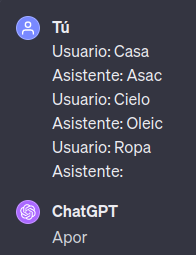
\includegraphics[width=0.2\textwidth]{./figuras/few_shot_prompting.png}
%     \source{Elaboración propia}
%     \label{fig:few_shot_prompting}
% \end{figure}


\begin{figure}[H]
    \caption[Técnica de \textit{few-shot prompting}]{Técnica de \textit{few-shot prompting}. El LLM recibe como input una serie de pares <<petición-respuesta>> más una petición a la cual ha de responder de forma análoga al contexto. En este caso, el LLM, con papel de <<asistente>>, ha de devolver el input del <<usuario>> con las letras invertidas. Sin embargo, nunca se le pide explícitamente que invierta las letras, sino que lo ha de inferir a partir de los ejemplos.}
    \centering
    \begin{subfigure}{.48\textwidth}
      \centering
      \begin{mdframed}
        Usuario: Casa
        \vspace{0.1cm}

        Asistente: Asac
        \vspace{0.1cm}

        Usuario: Ciclo
        \vspace{0.1cm}

        Asistente: Oleic
        \vspace{0.1cm}

        Usuario: Ropa
        \vspace{0.2cm}
      \end{mdframed}
    %   \caption{Csound}
    \end{subfigure}\hfill

    \vspace{0.2cm}

    \begin{subfigure}{.48\textwidth}
        \centering
        \begin{mdframed}
        Asistente: Apor
        \end{mdframed}
      \end{subfigure}\hfill

      \source{Elaboración propia}
      \label{fig:few_shot_prompting}
\end{figure}

\subsubsection{\textit{Chain of thoughts}}

Una técnica muy interesante es la denominada \gls{cot}, que consiste en presentar al \gls{llm} un problema y pedirle que explique su razonamiento antes de dar la respuesta. Esta técnica se ha mostrado muy efectiva en especial en tareas de resolución de problemas aritméticos, ya que obliga al \gls{llm} a razonar antes de dar una respuesta, lo que lleva a una respuesta correcta en la mayoría de los casos \citep{weiChainofThoughtPromptingElicits2023}. Esta técnica pone en evidencia el hecho de que los \gls{llm} no razonan necesariamente su respuesta, a pesar de que ésta pueda resultar conviencente y pasar por correcta (ver \ref{sec:limitaciones_llm}). Por otra parte, esta técnica ha mostrado que el \textit{prompting} tiene un gran poder sobre el resultado de la inferencia en los modelos de lenguaje. 

La Figura \ref{fig:chain_of_thoughts} muestra un ejemplo de \gls{cot} aplicado a un problema aritmético. Obsérvese cómo el \gls{llm} llega a la respuesta correcta sólo cuando se le incita a dar una explicación de su razonamiento. En este caso no se le ha pedido esta explicación explícitamente, sino a través de la técnica de \textit{few-shot prompting}. Las técnicas que se presentan a continuación pueden entenderse como derivaciones del principio de \gls{cot}, en los cuales se fuerza un razonamiento explícito por parte del \gls{llm} antes de dar una respuesta.

\begin{figure}[H]
    \caption[Chain of thoughts]{\textit{Chain of thoughts}. En ambos ejemplos se plantea un problema aritmético a GPT-3. En (a), por medio de \textit{few-shot prompting}, se le pide una respuesta directa al problema. En (b), aplicando, además, la técnica de \textit{chain of thoughts}, se le pide que explique su razonamiento, lo cual lleva a una respuesta correcta. Se ha resaltado el texto correspondiente a los razonamientos.}
    \centering
    \begin{subfigure}{.48\textwidth}
      \centering
      \begin{mdframed}
        \setstretch{1}
        P: Roger tiene 5 pelotas de tenis. Compra 2 latas más de pelotas de tenis. Cada lata tiene 3 pelotas de tenis. ¿Cuántas pelotas de tenis tiene ahora?
        \vspace{0.2cm}

        R: La respuesta es 11.
        \vspace{0.2cm}

        P: La cafetería tenía 23 manzanas. Si usaron 20 para hacer el almuerzo y compraron 6 más, ¿cuántas manzanas tienen?
        \vspace{0.2cm}
      \end{mdframed}
    %   \caption{Csound}
    \end{subfigure}\hfill
    \begin{subfigure}{.48\textwidth}
      \centering
      \begin{mdframed}
        \setstretch{1}
        P: Roger tiene 5 pelotas de tenis. Compra 2 latas más de pelotas de tenis. Cada lata tiene 3 pelotas de tenis. ¿Cuántas pelotas de tenis tiene ahora?
        \vspace{0.2cm}

        R: \highlight{Roger comenzó con 5 pelotas. 2 latas de 3 pelotas de tenis cada una hacen 6 pelotas de tenis. 5 + 6 = 11.} La respuesta es 11.
        \vspace{0.2cm}

        P: La cafetería tenía 23 manzanas. Si usaron 20 para hacer el almuerzo y compraron 6 más, ¿cuántas manzanas tienen?
        \vspace{0.2cm}
      \end{mdframed}
    %   \caption{SuperCollider}
    \end{subfigure}

    \vspace{0.2cm}

    \begin{subfigure}{.48\textwidth}
        \centering
        \begin{mdframed}
        R: La respuesta es 29.
        \end{mdframed}
        \caption{\textit{Few-shot} para forzar una resolución directa de un problema aritmético. La respuesta es incorrecta.}
      \end{subfigure}\hfill
    \begin{subfigure}{.48\textwidth}
      \centering
      \begin{mdframed}
        \setstretch{1}
        R: \highlight{Comenzaron con 23 manzanas. Usaron 20, por lo que quedaron 23-20 = 3 manzanas. Compraron 6 más, por lo que ahora tienen 3+6 = 9 manzanas.} La respuesta es 9.
      \end{mdframed}
      \caption{\textit{Few-shot} con \textit{chain of thoughts} para provocar un razonamiento previo a la respuesta. La respuesta es correcta.}
    \end{subfigure}

    \source{\cite{weiChainofThoughtPromptingElicits2023}. Traducción propia.}
    \label{fig:chain_of_thoughts}
\end{figure}

\subsubsection{\textit{Self Consistency of Chain of Thoughts}}

Esta técnica es una variante de \gls{cot} que consiste en presentar al \gls{llm} un problema y pedirle que explique su razonamiento antes de dar la respuesta, pero en este caso se le pide realizar esta cadena de pensamientos en dos o más ocasiones, Tras ello se verifica qué respuesta es la más consistente. De este modo, no solo se provoca el razonamiento, sino y la posibilidad de llegar a un resultado desde diferentes puntos de vista. \cite{wangSelfConsistencyImprovesChain2023} muestra cómo esta técnica mejora a la de \gls{cot} tanto en el terreno arimético como en el del razonamiento por sentido común. La Figura \ref{fig:cot_sc} muestra un ejemplo de esta técnica aplicada a un problema aritmético.

\begin{figure}[H]
    \caption[]{Esquema de los pasos en los que se divide la técnica \textit{Self Consistency of Chain of Thoughts}}
    \centering
    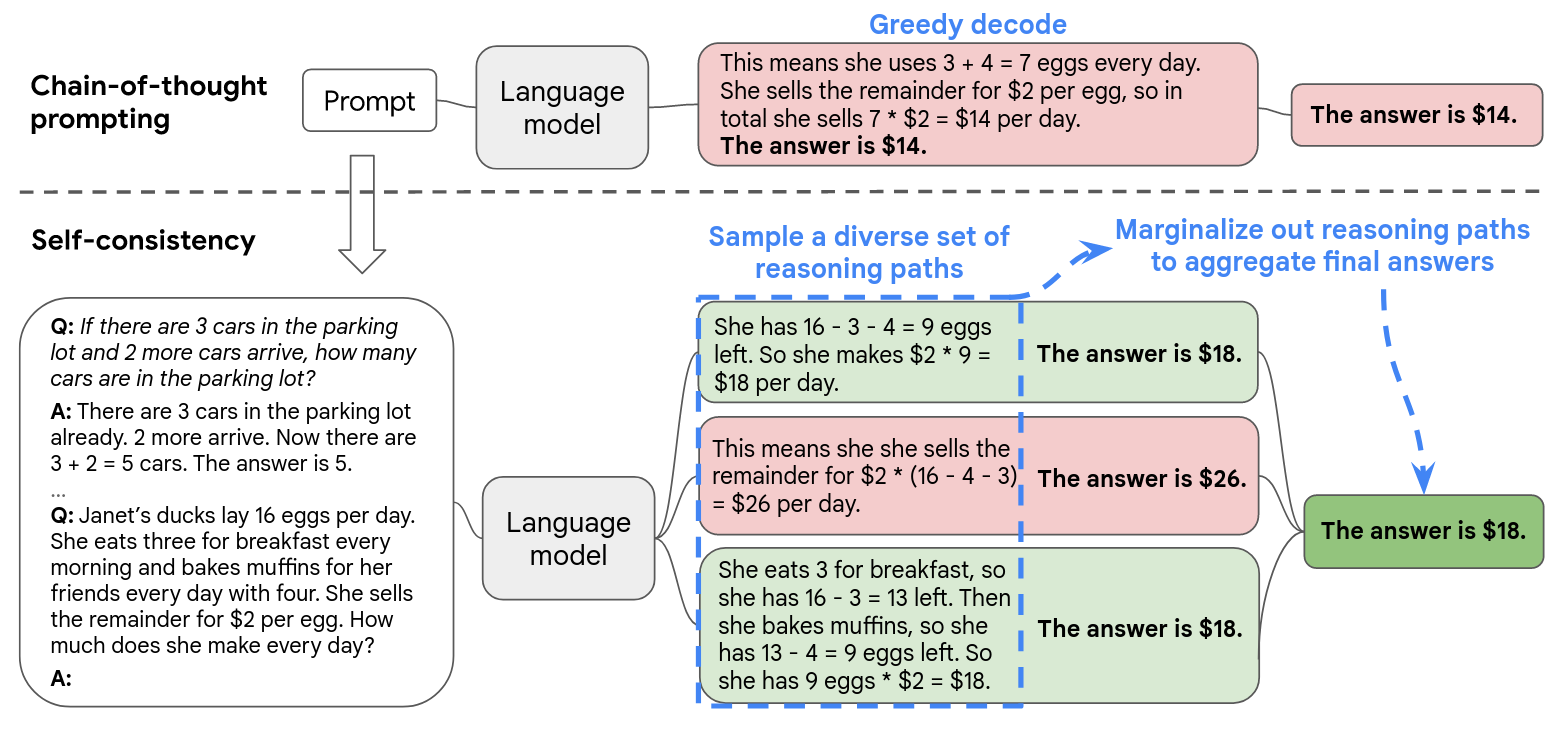
\includegraphics[width=0.9\textwidth]{./figuras/cot_sc.png}
    \source{\cite{wangSelfConsistencyImprovesChain2023}}
    \label{fig:cot_sc}
\end{figure}

\subsubsection{\textit{Tree of Thoughts}}

Esta técnica implementa un arbol de decisión. El \gls{llm} hace una búsqueda en profundidad y anchura en un arbol de pensamientos, pudiendo ir hacia atrás en la estructura si no encuentra una respuesta satisfactoria. La Figura \ref{fig:prompting_engineering} muestra un esquema de esta técnica comparada con la de \gls{cot} y \gls{cot_sc}.

\begin{figure}[H]
  \caption[Técnicas de \textit{prompting engineering}]{Técnicas de \textit{prompting engineering} aplicadas a problemas aritméticos.}
  \centering
  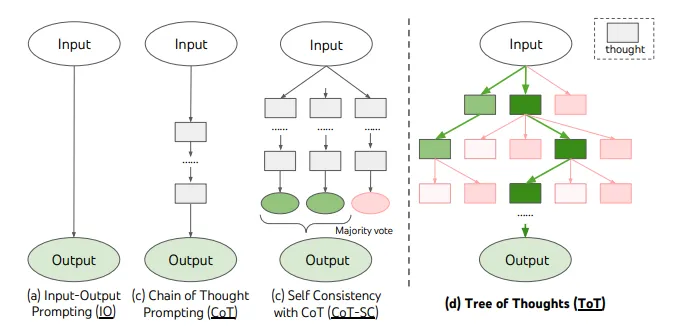
\includegraphics[width=0.9\textwidth]{./figuras/prompt_engineering_techniques.png}
  \source{\cite{bhavsarPromptEngineeringArithmetic2023}}
  \label{fig:prompting_engineering}
\end{figure}











El buen desempeño de los \gls{llm} en tareas de código de programación lleva a estudios como \cite{liStructuredChainofThoughtPrompting2023}, que propone un sistema de prompting que pide al \gls{llm} una reflexión explícita sobre la implementación a realizar, en una especie de pseudocódigo, que en un segundo paso será traducido al código final de programación. Este sistema de prompting se basa en la idea de que el \gls{llm} generará código de mayor calidad si se le permite <<pensar>> la respuesta antes de generarla. En este sentido, existen sobradas publicaciones que ponen de relieve la sensibilidad de los \gls{llm} a la forma en la que se le pide que procese la información (\textit{prompting}) y la correlación en la calidad de sus resultados \citep{zhouLeasttoMostPromptingEnables2023,weiChainofThoughtPromptingElicits2023,LLMPromptingGuide}.
 
\subsection{\textit{Retrieval-Augmented Generation}}

Los modelos de lenguaje están prentrenados con grandes cantidades de texto de propósito general, lo que los hace capaces y hábiles en multiples campos sin necesidad de un entrenamiento específico (ver Figura \ref{fig:fundation_models_habilities}). Es posible, sin embargo, rentrenarlos con datos más concretos y precisos para una tarea específica (por ejemplo, con datos médicos, ingenieriles, con datos privados de una empresa, etc.). A este proceso se le conoce como \textit{fine-tuning} o <<ajuste fino>>. Sin embargo, el proceso de \textit{fine-tuning} de un \gls{llm} requiere de grandes cantidades de datos y tiempo de entrenamiento, algo que en este momento no está al alcance del usuario medio. Por ello, se están desarrollando técnicas que permitan a los usuarios aprovechar los modelos preentrenados para tareas específicas sin necesidad de \textit{fine-tuning}. Una de estas técnicas es \gls{rag} \citep{WhatRetrievalaugmentedGeneration2021}, que podemos traducir por <<Generación Mejorada por Recuperación>>, que combina la recuperación de información con la generación de texto. Esta es una técnica que ofrece resultados muy notables en términos de eficacia y eficiencia frente al \textit{fine-tuning}. \gls{rag} consiste en pasar como contexto al \gls{llm} junto a la petición del usuario, una serie de fragmentos de texto que se corresponden semánticamente con la petición, y que se obtienen de una base de datos de documentos relacionados con la tarea a realizar. Esta base de datos puede ser de cualquier tipo, desde una base de datos de texto en lenguaje natural, hasta una base de datos de código de programación, pasando por una base de datos de partituras musicales, o una base de datos de audio, y representan la base de conocimiento extra (\textit{knowledge}) que el \gls{llm} manejará en sus interacciones con el usuario. Este sistema de \textit{prompting} está en la base actual de muchos productos relacionados con \gls{llm}, como Assistant o GPTs de OpenAI. La Figura \ref{fig:rag} muestra el esquema de funcionamiento de \gls{rag}. La base de datos del conocimiento del \gls{llm} es dividido en una primera fase en fragmentos más pequeños y analizados por el \gls{llm} para obtener una representación vectorial de cada uno de ellos. En una segunda fase, el \gls{llm} recibe el \textit{prompt} del usuario y lo analiza para obtener una representación vectorial. En una tercera fase, el \gls{llm} busca en la base de datos de fragmentos aquellos que tienen similitud vectoria (y, por ende, semántica) con el \textit{prompt} del usuario. En una cuarta fase, el \gls{llm} genera el texto de salida a partir del \textit{prompt} del usuario y de los fragmentos de texto recuperados de la base de datos. 



\begin{figure}[H]
    \caption[Esquema de funcionamiento de RAG]{Esquema de funcionamiento de \gls{rag}. El LLM recibe como input el \textit{prompt} del usuario y, como contexto, una serie de fragmentos de texto de la base de datos de conocimiento, que tienen similitud vectorial con el \textit{prompt} del usuario.}
    \centering
    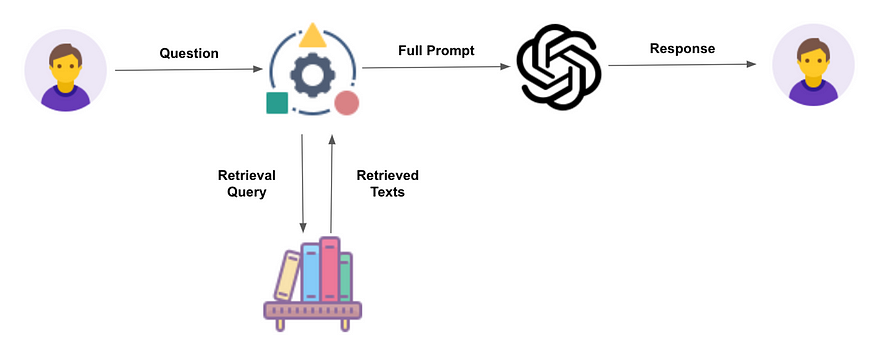
\includegraphics[width=0.9\textwidth]{./figuras/rag.png}
    \source{\cite{WhatRetrievalAugmented}}
    \label{fig:rag}
\end{figure}

Esta técnica, frente al \textit{fine-tuning}, ofrece una serie de ventajas, como la posibilidad de utilizar modelos preentrenados de propósito general, que son más eficientes y eficaces que los modelos entrenados para una tarea específica, y la posibilidad de utilizar bases de datos de conocimiento de gran tamaño, que son más fáciles de obtener que los grandes conjuntos de datos necesarios para el \textit{fine-tuning}. Además, la base de datos de conocimiento puede ser actualizada de forma independiente al modelo, lo que permite una mayor flexibilidad en el uso de los modelos. Por contra, el modelo no tiene conocimiento global de los contenidos de la base de datos, por lo que no puede realizar inferencias globales sobre ella, y la calidad de los resultados depende en gran medida de cómo se ha dividido su contenido en fragmentos y de la calidad de la representación vectorial de cada uno de ellos. Se ha probado un mayor rendimiento en técnicas combinadas de \textit{fine-tuning} para tareas específicas y \gls{rag} \citep{lewisRetrievalAugmentedGenerationKnowledgeIntensive2021}.


\subsubsection{\textit{prompting} versus \textit{fine-tuning} versus \textit{Retrieval-Augmented Generation}}

Seguimos a \cite{arunbijiRAGVsFinetuning}


\subsection{Habilidades emergentes de los modelos de lenguaje}

\begin{figure}
    \caption{Habilidades de los \textit{Foundation Models} de OpenAI.}
    \centering
    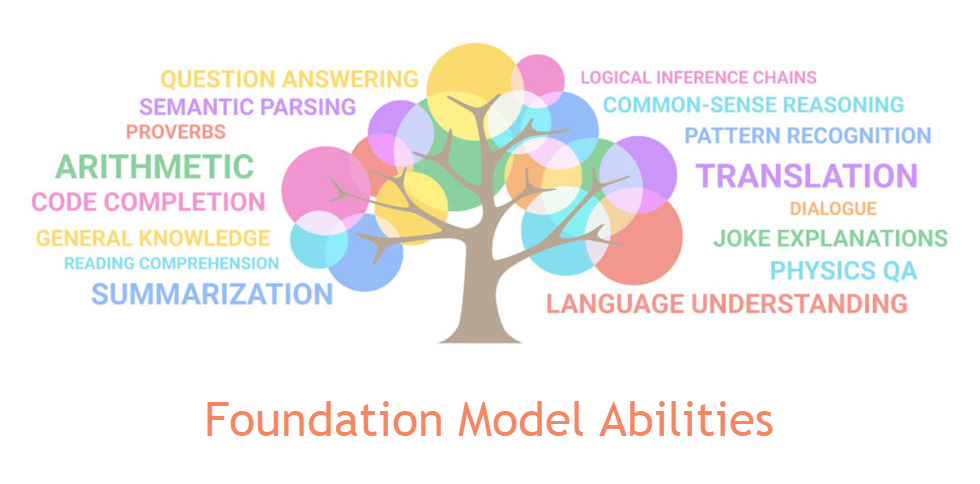
\includegraphics[width=0.8\textwidth]{./figuras/fundation_models_habilities.png}
    \source{\cite{GPT3RiseFoundation}}
    \label{fig:fundation_models_habilities}
\end{figure}
